% command to make sure colorboxes don't create whitespace between code lines
\fboxsep=.6pt

% default settings for listings
\lstset{style=python}

\title[Textverarbeitung in \LaTeX\ Teil 1]{Textverarbeitung in \LaTeX\ Teil 1}

\subtitle{\LaTeX}

\author[Graf, Thomas] % (optional)
{Thomas Graf}

\institute[KLW] % (optional)
{
    Fachschaft Informatik\\
    Kantonsschule im Lee
}

\date[\today] % (optional)

\logo{
\includegraphics[width=2cm]{Logos/LeeLogo}}

\titlegraphic{\vspace{-.7cm}\includegraphics[width=\textwidth]{"Grundlagen_Info/06_Datenbanken/Figures/title-emojis"}}

\frame{\titlepage}


\begin{frame}[fragile]
\frametitle{Was ist \LaTeX?}
	\begin{columns}
		\begin{column}{0.3\textwidth}
			\vspace{\topsep}
			
\includegraphics[scale=0.12]{EF/LaTeX/Slides/latex_logo.pdf}
		\end{column}
		\begin{column}{0.65\textwidth}
			\begin{itemize}[<+->]
				\item Textverarbeitungssoftware
				\item sehr gut geeignet zur Verfassung von:
				      \begin{itemize}[<+->]
					      \item Maturitätsarbeiten
					      \item Bachelorarbeiten / Masterarbeiten
					      \item Beamer Präsentationen (Slides)
					      \item wissenschaftliche Publikationen
					      \item Büchern
				      \end{itemize}
			\end{itemize}
		\end{column}
	\end{columns}
\end{frame}


\begin{frame}[fragile]
	\frametitle{Korrekte Aussprache von \LaTeX}
	\begin{columns}
		\begin{column}{0.3\textwidth}
			\vspace{\topsep}
			
\includegraphics[scale=0.09]{EF/LaTeX/Slides/chi.png}
		\end{column}
		\begin{column}{0.65\textwidth}
			Das \textcolor{Red}{X} im Wort \LaTeX\ ist kein grosses X wie im Wort \textit{Xylophon}, sondern der gross geschriebene griechische Buchstabe Chi.

			Die Aussprache von Chi ist ein hartes \textit{ch}, so wie im deutschen Wort \textit{a\textbf{ch}}.

			Deshalb ist die Aussprache von \LaTeX\ nicht Late\textbf{x}, sondern \textcolor{NavyBlue}{Late\textbf{ch}}. (Latex ist der Milchsaft verschiedener Kautschukpflanzen und hat mit Textverarbeitung wenig zu tun.)
		\end{column}
	\end{columns}
\end{frame}


\begin{frame}[fragile]
	\frametitle{Unterschiede zwischen MS Word und \LaTeX }
	Man unterscheidet (grob) zwischen zwei Kategorien von Textverarbeitungssoftware:
	\begin{itemize}[<+->]
		\item WYSIWYG
		\item WYSIWYM
	\end{itemize}
\end{frame}


\begin{frame}[fragile]
	\frametitle{WYSIWYG}
	\textbf{WYSIWYG} (\enquote{\textcolor{Red}{W}hat \textcolor{Red}{Y}ou \textcolor{Red}{S}ee \textcolor{Red}{I}s \textcolor{Red}{W}hat \textcolor{Red}{Y}ou \textcolor{Red}{G}et})

	\begin{itemize}[<+->]
		\item 
	Bei (echtem) WYSIWYG wird ein Dokument während der Bearbeitung am Bildschirm genauso angezeigt, wie es bei der Ausgabe über ein anderes Gerät, z.B. einen Drucker, aussieht. ($\rightarrow$ Echtzeitdarstellung)
		\item 
	bekannte Beispiele: MS Word, MS PowerPoint, Gmail, WhatsApp
	\end{itemize}
\end{frame}


\begin{frame}[fragile]
	\frametitle{WYSIWYM}
	\textbf{WYSIWYM} (\enquote{\textcolor{NavyBlue}{W}hat \textcolor{NavyBlue}{Y}ou \textcolor{NavyBlue}{S}ee \textcolor{NavyBlue}{I}s \textcolor{NavyBlue}{W}hat \textcolor{NavyBlue}{Y}ou \textcolor{NavyBlue}{M}ean})

	\begin{itemize}
		\item 
	Am Bildschirm ist während der Eingabe für den Benutzer nur in etwa erkennbar, was er mit seiner Formatierung bezwecken will.
		\item
	Die endgültige Formatierung wird erst beim Umwandeln des Dokuments in ein Endformat (z.B. PDF) durchgeführt.
		\item
	bekannte Beispiele: \LaTeX, (X)HTML, CSS
	\end{itemize}
\end{frame}

\begin{frame}[fragile]
	\frametitle{kleiner Joke ...}
\begin{center}
    
\includegraphics[scale=0.15]{EF/LaTeX/Slides/word_vs_latex.jpg}
\end{center}
\end{frame}


\begin{frame}[fragile]
\frametitle{Lokale Installation (auf eigenem Rechner)}
Benötigt werden typischerweise
\begin{itemize}[<+->]
    \item eine \TeX-Distribution (TeX Live, MacTex, MiKTex, ...)
    \item ein geeigneter \TeX-Editor (z.B. VSCode, TeXstudio, TEXMAKER)
\end{itemize}
\end{frame}


\begin{frame}[fragile]
\frametitle{Installation einer \TeX-Distribution}
\begin{itemize}[<+->]
    \item MacOS:
\begin{lstlisting}[language=bash, numbers=none]
brew install --cask mactex
\end{lstlisting}
\item Windows:
\begin{lstlisting}[language=bash, numbers=none]
winget install --id MiKTeX.MiKTeX
winget install --id StrawberryPerl.StrawberryPerl
\end{lstlisting}
\item Starte deinen Computer neu.
\end{itemize}
\end{frame}

\begin{frame}[fragile]
	\frametitle{Installation und Konfiguration einer \LaTeX-Extension für VSCode}
	Installiere die VSCode-Extension \texttt{Latex Workshop} (von James Yu).
\end{frame}

\begin{frame}[fragile]
	\frametitle{Latex Workshop Rezepte erstellen}
	Öffne in VSCode die Kommando-Palette durch:
\begin{itemize}[<+->]
    \item MacOS:
\begin{lstlisting}[language=bash, numbers=none]
Cmd + Shift + P
\end{lstlisting}
\item Windows:
\begin{lstlisting}[language=bash, numbers=none]
Ctrl + Shift + P
\end{lstlisting}
\end{itemize}
und tippe: \texttt{Preferences: Open User Settings (JSON)}. Dies sollte das File \texttt{settings.json} öffnen.

\textbf{Fügen} Sie den Code in \texttt{latex\_recipies.json} (siehe Moodle) zu Ihrem \texttt{settings.json} hinzu.
\end{frame}

\begin{frame}[fragile]
\frametitle{erstes Dokument}
	    Erstellen Sie in VSCode ein neues File \texttt{minimal.tex} mit dem folgenden Inhalt:
		\lstinputlisting[style=LaTeX,caption=\texttt{minimal.tex},label=listing:minimal]{EF/LaTeX/Slides/Code/minimal.tex}
	    % \begin{lstlisting}[style=LaTeX]
	    %     \documentclass{article}
	        
	    %     \begin{document}
	    %     Hello, World!
	    %     \end{document}
	    % \end{lstlisting}
		und kompilieren Sie dieses mit der Extension \texttt{Latex Workshop}.
\end{frame}

\begin{frame}[fragile]
\frametitle{Befehle (commands) in \LaTeX}
\begin{lstlisting}[style=LaTeX,basicstyle=\footnotesize\ttfamily]
\NameDesBefehls % Befehl ohne Argumente und ohne Optionen
\NameDesBefehls{} % mit einem Argument
\NameDesBefehls[]{} % mit Optionen und einem Argument
\NameDesBefehls[]{}{} % mit Optionen und 2 Argumenten
\end{lstlisting}
\end{frame}

\begin{frame}[fragile]
\frametitle{Beispiele von Befehlen in \LaTeX}
\begin{itemize}[<+->]
    \item \lstinline[style=LaTeX]|\textbf{Jane Doe}| (setzt \textit{Jane Doe} in Fettschrift)
    \item \lstinline[style=LaTeX]|{\huge Hallo}| (macht \textit{Hallo} sehr gross)
    \item \lstinline[style=LaTeX]|\today (setzt das aktuelle Datum)|
    \item \lstinline[style=LaTeX]|\section{neuer Abschnitt}| (erstellt einen neuen Abschnitt)
    \item \lstinline[style=LaTeX]|\documentclass[a4paper,12pt]{article}| {\small (setzt die Dokumentklasse auf \textit{article}, das Format auf A4 und die Textgrösse auf 12pt)}
    \item \lstinline|\textcolor{Red}{roter Text}| {\small (färbt \textit{roter Text} rot)}
\end{itemize}
\end{frame}

\begin{frame}[fragile]
\begin{myexercise}\label{myexercise:hitchens-razor}
    Erstellen Sie ein PDF-Dokument mit exakt folgendem Inhalt (recherchieren Sie):
    
        \begin{center}
            \textbf{What can} be asserted \underline{witho}ut evidence can also be \textit{dismissed} without evi\underline{denc}e.
        \end{center}
\end{myexercise}
\end{frame}


\begin{frame}[fragile]
\frametitle{Pakete}
\begin{lstlisting}[style=LaTeX]
\usepackage{NameDesPakets}
\usepackage[Zusatzoptionen]{NameDesPakets}
\end{lstlisting}

Alle \lstinline[style=LaTeX]|\usepackage{...}| Befehle müssen \textbf{nach} \lstinline[style=LaTeX]|\documentclass{...}| und \textbf{vor} \lstinline[style=LaTeX]|\begin{document}| stehen!

\vspace{1cm}
wichtige Informationsquelle: \url{https://ctan.org/}
\end{frame}

\begin{frame}[fragile]
\frametitle{Umgebungen (environments) in \LaTeX}
\begin{lstlisting}[style=LaTeX,breaklines,numbers=left,tabsize=2]
\begin{NameDerUmgebung}
Hier soll etwas Interessantes geschehen.
\end{NameDerUmgebung}
\end{lstlisting}
Beispiele:
\begin{lstlisting}[style=LaTeX]
\begin{itemize}
	\item erster Bulletpunkt
	\item zweiter Bulletpunkt
\end{itemize}

% Ausnahme: Formel-Environment mit Dollar-Zeichen $$ (oder ähnliche)
$\alpha + 4 = \gamma -2$
\end{lstlisting}
\end{frame}


\begin{frame}[fragile]
\begin{myexercise}\label{myexercise:pythagoras}
    Recherchiere im Internet, um folgendes in \LaTeX\ sinngemäss zu reproduzieren:
    \begin{itemize}
        \item Pythagoras: $a^2 + b^2 = c^2$
        \item $\Rightarrow c = \sqrt{a^2 + b^2}$
    \end{itemize}
    Symbole und Formeln müssen zwischen Dollar-Zeichen geschrieben werden: \lstinline[style=LaTeX]|$ ... $|.
\end{myexercise}
\end{frame}

\begin{frame}[fragile]
\frametitle{Beispiel: Bilder in \LaTeX\ einfügen}
\begin{lstlisting}[style=LaTeX, numbers=left, tabsize=2]
\begin{figure}
    \centering
    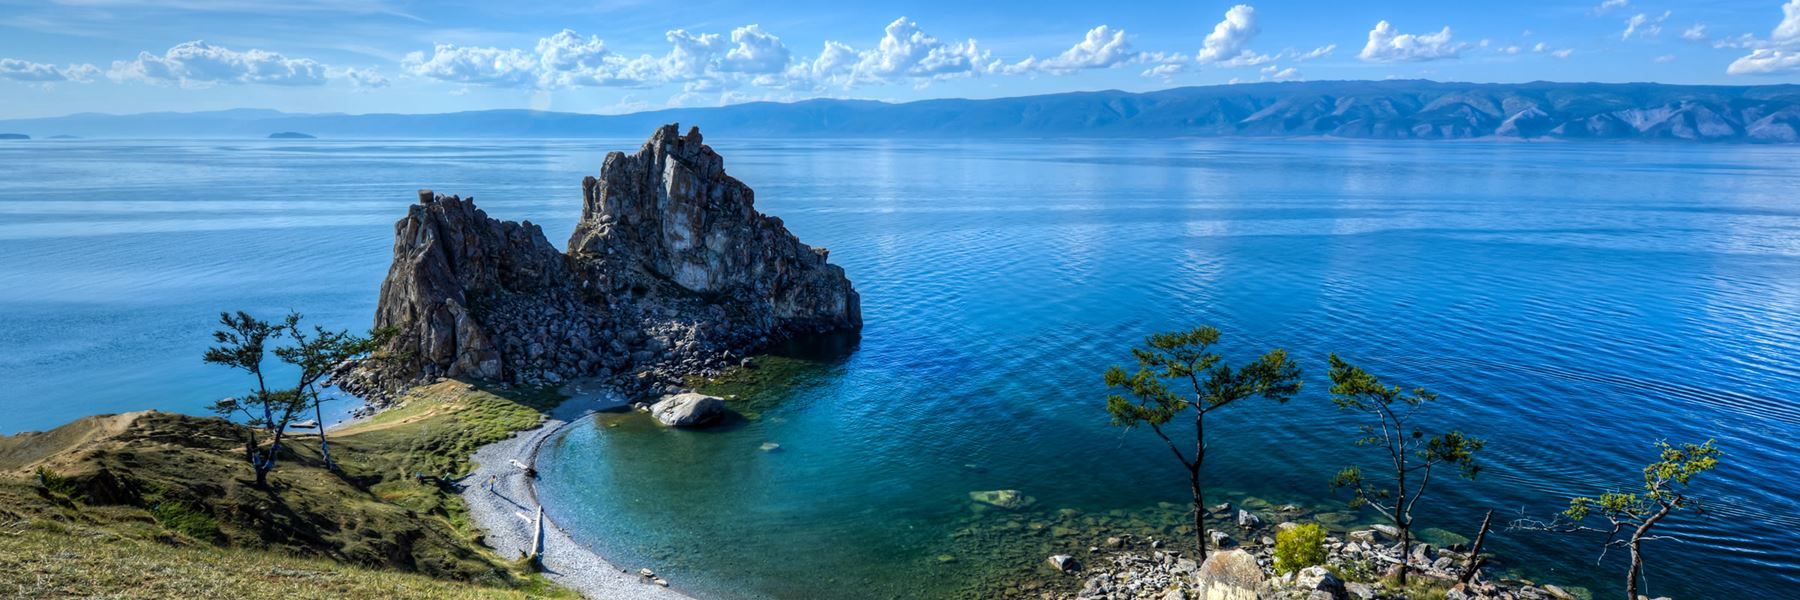
\includegraphics[width=0.7\textwidth]{baikal.jpg}
    \caption{Baikalsee}
\end{figure}
\end{lstlisting}
benötigt \lstinline[style=LaTeX]|\usepackage{graphicx}|

\begin{figure}
    \centering
    
\includegraphics[width=0.7\textwidth]{EF/LaTeX/Slides/baikal.jpg}
    \caption{Baikalsee}
\end{figure}
\end{frame}

\begin{frame}[fragile]
\begin{myexercise}\label{myexercise:image-caption}
Speichern Sie ein Bild Ihrer Wahl in demselben Ordner wie Ihr \LaTeX-Dokument ab. Skalieren Sie das Bild angemessen und geben Sie ihm eine kurze Beschreibung in blauer Farbe.
\begin{figure}
    \centering
    
\includegraphics[width=0.6\textwidth]{EF/LaTeX/Slides/saltwater_crocodile.jpg}
    \caption{\textcolor{blue}{Salzwasserkrokodil an Strand in Darwin, Australien}}
    \label{fig:crocodile}
\end{figure}
\end{myexercise}
\end{frame}


\begin{frame}[fragile]
\begin{myexercise}
Informiere Dich über das \lstinline[style=LaTeX]|align| Environment und mathematische Formeln in \LaTeX\ im Internet und versuche folgende Ausdrücke zu reproduzieren:
\begin{align}
e^{i\pi}+1 &= 0\\
&\sqrt[4]{8}\\
(x+y)^n &= \sum_{r=0}^n\binom{n}{r}x^r y^{n-r}
\end{align}
\end{myexercise}
\end{frame}


\begin{frame}[fragile]
\begin{myexercise}
\textcolor{red}{Griechisch}\\
Informationen über das griechische Alphabet:
\begin{enumerate}
    \item Der erste Buchstabe des griechischen Alphabets ist $\alpha$.
    \item Das Alphabet umfasst \underline{24} Buchstaben.
\end{enumerate}

\begin{lstlisting}[style=LaTeX, basicstyle=\scriptsize\ttfamily]
\documentclass{article}
\begin{document}
\usepackage{xcolor}
\indent
\textcolor{red}{Griechisch}
Informationen über das griechische Alphabet:
\begin{itemize}
    \item Der erste Buchstabe des griechischen Alphabets ist \alpha.
    \item Das Alphabet umfasst \underscore{24} Buchstaben.
\end{itemize}
\end{lstlisting}
Finde mindestens vier Fehler im obigen \LaTeX-Dokument.
\end{myexercise}
\end{frame}


\begin{frame}[fragile]
\begin{myexercise}
    \begin{enumerate}
        \item Erstelle im Table-Generator \url{https://www.tablesgenerator.com/} eine Tabelle mit 3 Zeilen und 4 Spalten und fülle die Einträge mit beliebigen Zahlen. Füge die dabei entstandene Tabelle in ein \LaTeX-Dokument ein und betrachte das Resultat.
        \item Versuche den AI-Coding Assistenten eine gleichartige Tabelle erstellen zu lassen. Welches Vorgehen scheint dir einfacher?
    \end{enumerate}
\end{myexercise}
\end{frame}

\begin{frame}[fragile]
\frametitle{Historische Entwicklung}
\TeX\ ist ein im Jahre 1978 veröffentlichtes Computerprogramm zur Erstellung von digitalen Texten, welches hauptsächlich von dem berühmten US-amerikanischen Informatiker Donald E. Knuth geschrieben wurde. Sein Hauptziel war es, mit \TeX\ ein Werkzeug zu schaffen, mit dessen Hilfe hochqualitative Bücher mit wenig Aufwand verfasst werden können. Des weiteren sollte \TeX\ auf jedem Computer und zu jeder Zeit identische Resultate (Texte) produzieren \footnote{Details zur Geschichte von \TeX\ findet man hier: \url{https://www.tug.org/whatis.html}}.
\end{frame}


\begin{frame}[fragile]
\frametitle{Entwicklung von \TeX}
\begin{center}
    
\includegraphics[scale=0.5]{EF/LaTeX/Slides/knuth.jpg}
    \captionof{figure}{Donald Ervin Knuth}
\end{center}
\end{frame}


\begin{frame}[fragile]
\frametitle{Historische Entwicklung}
\TeX\ ist insbesondere eine Programmiersprache. Diese ermöglicht die Definition diverser Befehle, welche den Computer z.B. beauftragen, die Schriftgrösse anzupassen, Abstände im Text einzubauen oder die Schriftart zu ändern. Eine \TeX-Distribution enthält viele solcher bereits definierten primitive Befehle. Ein Beispiel eines solchen Befehls ist \lstinline[style=LaTeX]{\baselineskip = 24pt}, welcher bewirkt, dass zwischen den einzelnen Zeilen im Text ein Abstand von 24 Einheitspunkten gesetzt wird (in \TeX\ beginnen Befehle mit einem Backslash \lstinline|\\|).
\end{frame}


\begin{frame}[fragile]
\frametitle{Historische Entwicklung}
Nehmen wir an, wir möchten nun eine Präsentation wie diese hier schreiben. Konzentrieren wir uns einmal auf die Überschrift ``Historische Entwicklung'' dieses Abschnitts (Section). Wie ist diese wohl entstanden? 
Um eine solche Überschrift in \TeX\ zu erstellen, müssten dem Computer diverse Instruktionen (Befehle) übergeben werden:
\begin{itemize}
\item Befehle zur Anpassung der Schriftgrösse und Dicke der Schrift
\item diverse Befehle zum Einfügen bestimmter Abstände vor und nach der Überschrift
\item die blaue Färbung
\item usw.
\end{itemize}
\end{frame}

\begin{frame}[fragile]
\frametitle{Historische Entwicklung}
Dies bedeutet, dass wir zahlreiche \TeX-Befehle geschickt kombinieren müssten, um einen neuen Abschnitt deklarieren zu können. Dies erscheint recht unpraktisch zu sein. Was wäre jedoch, wenn jemand sich die Mühe machen würde, so einen komplexen Befehl für das Erstellen eines neuen Textabschnittes aus primitiven \TeX-Befehlen zusammenzusetzen? Diese tatkräftige Person könnte der Kombination aller dafür benötigten primitiven Befehle einen neuen Namen, wie z.B. \lstinline[style=LaTeX]|\section{}| geben. Dieser Befehl steht dann als Stellvertreter für die Kombination aller Befehle, welche zur Erstellung eines neuen Abschnitts notwendig sind. Man bezeichnet den dadurch entstandenen neuen Befehl als \textit{Makro} (griechisch $\mu\alpha\kappa\rho\acute{o}\sigma$ makros = `gross', `weit', `lang').
\end{frame}


\begin{frame}[fragile]
\frametitle{Historische Entwicklung}
Die Idee hinter Makros ist simpel und effektiv: man fasst alle kleinen (mikro) Befehle, welche benötigt werden, um z.B. einen neuen Abschnitt (Section) zu erstellen, zu einem neuen, grossen (makro) Befehl zusammen und gibt diesem einen Namen, wie beispielsweise \lstinline[style=LaTeX]|\section{}|. Dass dieses Vorgehen möglich ist, dürfte nicht erstaunen, da \TeX\, wie bereits erwähnt, eine vollwertige Programmiersprache ist, mit welcher natürlich solche neuen Befehle definiert werden können.
\subsubsection{\LaTeX}
\end{frame}


\begin{frame}[fragile]
\frametitle{Historische Entwicklung}
Der beflissene US-amerikanische Informatiker Leslie B. Lamport baute am Anfang der 1980er Jahre zahlreiche höchst nützliche Makro-Befehle aus primitiven \TeX-Befehlen zusammen. Das daraus resultierende Softwarepaket, welches die Benutzung von \TeX\ mit Hilfe von Makros stark vereinfacht, nennt sich \LaTeX\ (kurz für \textbf{La}mport \textbf{TeX}). \LaTeX\ ist also nichts anderes als eine auf \TeX\ aufbauende (und in \TeX\ geschriebene) Erweiterung von \TeX. Mittlerweile gibt es tausende von \TeX-Paketen, welche von diversen Leuten verfasst wurden und eine ungeheure Vielfalt an nützlicher Funktionalität zur \TeX\ / \LaTeX\ Basisdistribution
hinzufügen \footnote{umfangreiche Sammlung von \TeX-Paketen: \url{https://ctan.org/?lang=en}}. \LaTeX\ ist eine sogenannte \textit{freie Software} und unterliegt den Regelungen der LaTeX Project Public License (LPPL) \footnote{Details zur LPPL-Lizenz: \url{https://www.latex-project.org/lppl/}}.
\end{frame}


\begin{frame}[fragile]
\frametitle{Entwicklung von \LaTeX}
\begin{center}
    
\includegraphics[scale=0.5]{EF/LaTeX/Slides/lamport.jpg}
    \captionof{figure}{Leslie Lamport}
\end{center}
\end{frame}

\begin{frame}[fragile]
\frametitle{Macros in \LaTeX\ (ohne Argumente)}
In einem Laborbericht erwähnen wir häufig den vollen Namen von TNT, nämlich \textbf{2-Methyl-1,3,5-trinitrobenzen} (in Fettschrift). Dazu müsste man an den entsprechenden Stellen jeweils den Command \lstinline[style=LaTeX]|\textbf{2-Methyl-1,3,5-trinitrobenzen}| hinschreiben. Wenn man dies oft tun muss, ist es einfach, diesen Command durch ein Makro zu ersetzen, welchem wir den Namen \lstinline[style=LaTeX]|\TNT| geben möchten:

\begin{lstlisting}[style=LaTeX, basicstyle=\footnotesize\ttfamily]
    \newcommand{\TNT}{\textbf{2-Methyl-1,3,5-trinitrobenzen}}
\end{lstlisting}

\end{frame}

